\section{Data Analysis}
\subsection{Analyzing Window Size}

The findings on how window size influences classifier performance on both on the INRIA and Caltech data sets quite closely conforms to to the findings of the original authors. A higher sized window size captures more contextual information about the pedestrian and the surrounding area \cite{dalal_2005_histograms}, thus it is not surprising that the largest window size of (128, 96) outperformed all other window sizes in both INRIA and Caltech, as evident in figures \ref{fig:window_size_inria} and \ref{fig:window_size_caltech}. The PnPLO dataset, however, did not follow this trend, with the the two smallest windows ((112,48) and (100, 50)) dominating performance scores. This is likely due to to the fact that the smaller windows are able to focus more on local features rather than global context, reducing the amount of potentially "confusing" information. It may also be the case that greater window sizes cause the classifier to overfit to the artificial characteristics of mannequins and statues, like display platforms, causing worse performance on an independent test data set.


% Noting how this could inform practical applications - for example, a security system might want larger windows for detecting real pedestrians, while a museum inventory system cataloging statues might benefit from smaller windows

\subsection{Analyzing Derivative Masks}

The holistic derivative mask (HDM) proposed in section \ref{sec:deriv_mask} extraordinarily improved performance on both Caltech (figure \ref{fig:hdm_caltech}) and PnPLO (figure \ref{fig:hdm_pnplo}) data sets, with almost every configuration with HDM outperforming their counterpart without HDM (figure \ref{fig:hdm_total}). The HDM approach preserves gradient information at the boundaries where pedestrians might be visible, making use of limited pixel pixel information, which is especially important in low resolution images like those in the Caltech dataset \cite{dollar_2009_pedestrian}. The difference in performance on the INRIA data set appears to be less pronounced (figure \ref{fig:hdm_inria}), which isn't surprising given that pedestrians in INRIA are usually centered or at least have a significant amount of margin space around them \cite{dalal_2005_histograms}. Even so, the best performant INRIA configuration with HDM still outperforms the best performant configuration without HDM with statistical significance ($p=6\cdot 10^{-9}$), as shown in figure \ref{fig:best_hdm_inria}

\begin{figure}
    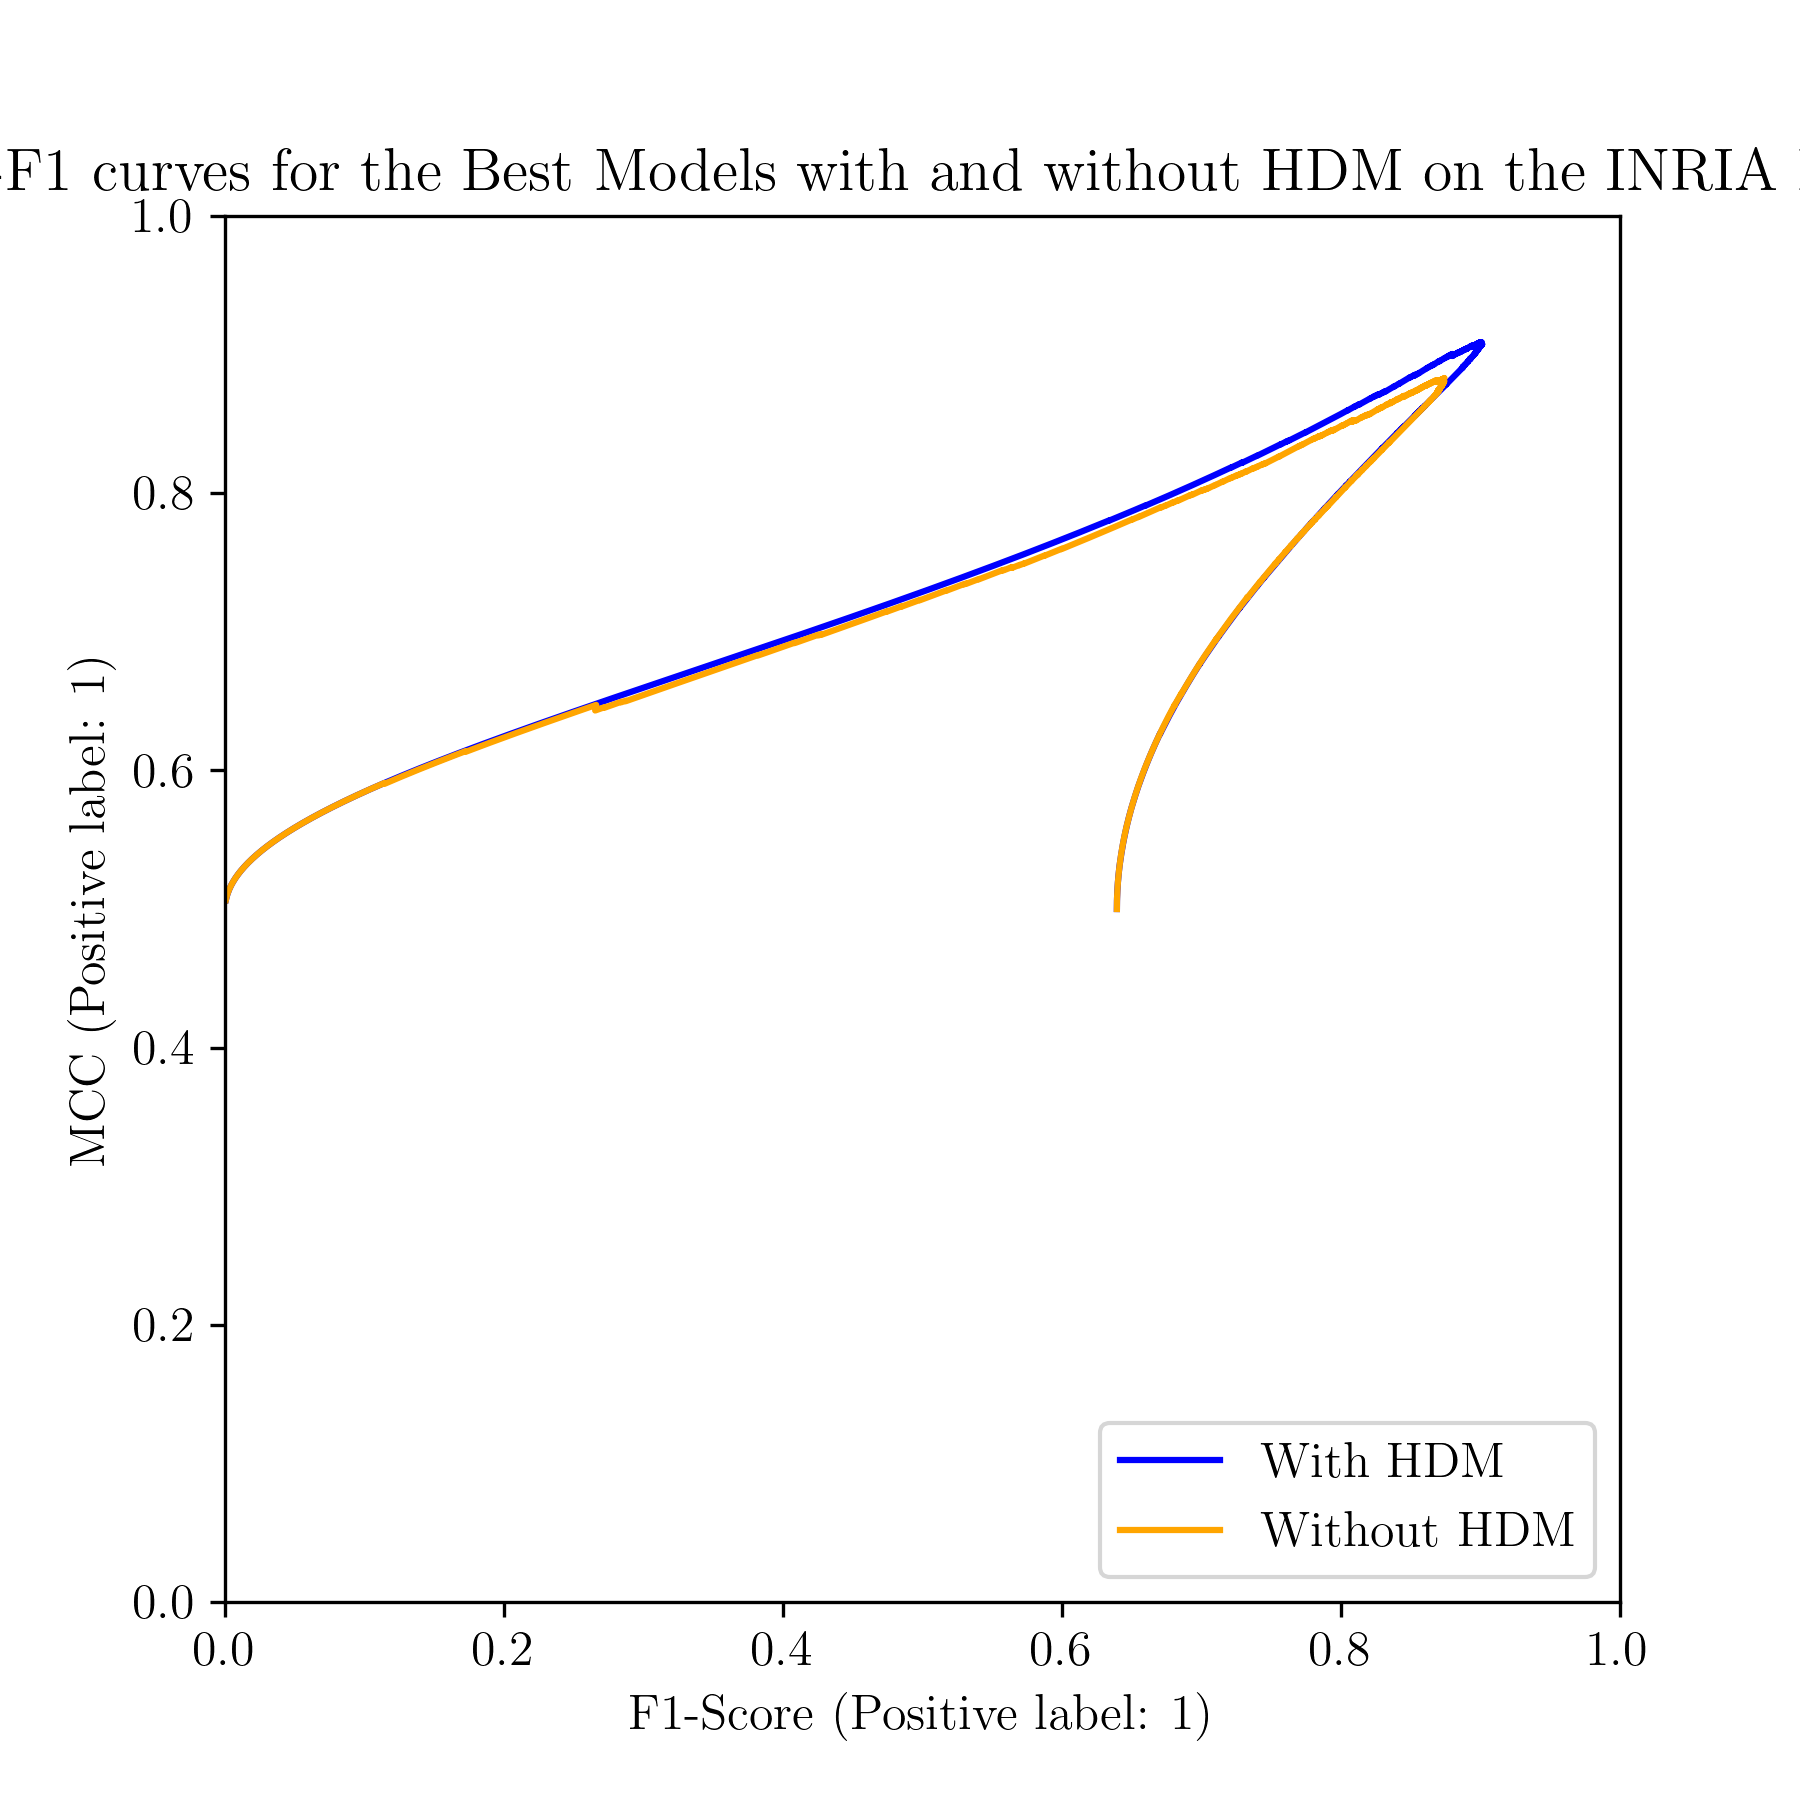
\includegraphics[width=0.6\linewidth]{best_hdm_mcc_f1_inria.png}
    \caption{
        The best performing configurations on the INRIA data set with and without the holistic derivative mask (HDM). 
    }
    \label{fig:best_hdm_inria}
\end{figure}


\subsection{Analyzing Orientation Bin Sizes}

The experimental results shown in Figures \ref{fig:orientation_bins_inria} through \ref{fig:orientation_bins_total} align with Dalal and Triggs' seminal HOG paper \cite{dalal_2005_histograms}: increasing the number of orientation bins beyond 9 yields minimal performance improvements (all pairwise p-values $\sim 0.05$). This demonstrates the law of diminishing returns in pedestrian detection, which can be attributed to the relatively consistent edge orientations in human body shapes. Finer orientation binning over the 0°-180° range (such as 13.8° intervals for 13 bins or 10° intervals for 18 bins) fails to capture significantly more discriminative information. While increasing bin count raises feature vector dimensionality (discussed in section \ref{sec:feature_vector_dimensionality}), which could theoretically degrade performance, our experiments show no such negative impact. In fact, configurations with 18 bins show marginally better performance than those with fewer bins, though this improvement is less influential than parameters such as window size or derivative mask selection.

\subsection{Analyzing Cell Size}


\subsection{Analyzing Block Density}